\documentclass[a4paper,openright,12pt]{article}

% Font config
\usepackage[utf8]{inputenc}
\usepackage{lmodern}
\usepackage[T1]{fontenc}
\usepackage{amsfonts}
\usepackage[babel=true]{microtype}
\usepackage{inconsolata}

% Figures, graphics, etc
\usepackage{graphicx}
\usepackage{caption}
\usepackage{subcaption}
\usepackage{float}

% Math symbols
\usepackage[mathscr]{eucal}
\usepackage{amsmath}
\usepackage{amssymb}

% Document Personalization and Language Configuration
\usepackage[spanish,es-noshorthands]{babel}
\usepackage{vmargin}
\usepackage{eurosym} 
\usepackage{xcolor}
\usepackage[export]{adjustbox}
\usepackage[document]{ragged2e}
\usepackage[shortlabels]{enumitem}

% Misc
\usepackage{titling}
\usepackage{titlesec}
\usepackage{afterpage}
\usepackage{csquotes}
\usepackage{multirow}
\usepackage{xurl}
\usepackage{hyperref}
\usepackage{listings}
\usepackage{array}
\usepackage{datetime}
\usepackage{mfirstuc}
\usepackage{multicol}
\usepackage{appendix}
\usepackage{glossaries} % Glossaries needs perl for makeglossaries. *NIX preinstalled. Windows: Strawberry Perl (choco install strawberryperl)

% Special
\usepackage{minted} % Minted needs python installed, and pygments on path [https://pypi.org/project/Pygments/]

% Configurations
\setcounter{secnumdepth}{4}
\setlist[enumerate]{itemsep=0mm}
\setlist[itemize]{itemsep=0mm}
\captionsetup{justification=centering,margin=2cm}
\setlength{\columnsep}{0.5cm}

% Anexos en español
\addto\captionsspanish{
  \renewcommand\appendixname{Anexo}
  \renewcommand\appendixpagename{Anexos}
  \renewcommand{\appendixtocname}{Anexos}
}

% No hyphenate
\usepackage[none]{hyphenat}
\sloppy

% Packages for FSM and diagrams
\usepackage{pgf}
\usepackage{tikz}
\usetikzlibrary{arrows,automata}

% Packages for generation mock images
\usepackage{duckuments}

% Things for Morse
\newcommand{\punto}{\kern+0.3pt\raisebox{0.35ex}{\huge\textbf.}}
\newcommand{\raya}{\kern+0.2pt\raisebox{-0.35ex}{\huge\textbf-}}
\usepackage[backend=biber, style=authoryear, backref=true, hyperref=true, urldate=long]{biblatex}
\addbibresource{bibliography.bib}
\addbibresource{bibliography.bib}

\setpapersize{A4}       %  DIN A4
\setmargins{3cm}        % margen izquierdo
{2cm}                   % margen superior
{15cm}                  % anchura del texto
{22.5cm}                % altura del texto
{10pt}                  % altura de los encabezados
{1cm}                   % espacio entre el texto y los encabezados
{0pt}                   % altura del pie de página
{2cm}                   % espacio entre el texto y el pie de página

\renewcommand{\labelenumii}{\theenumii}
\renewcommand{\theenumii}{\theenumi.\arabic{enumii}.}

\makeglossaries

\newglossaryentry{RISC}
{
    name={RISC},
    description={Reduced Intruction Set Computer}
}

\newglossaryentry{CISC}
{
    name={CISC},
    description={Complex Intruction Set Computer}
}

\newglossaryentry{ARM}
{
    name={ARM},
    description={Advanced RISC Machine}
}

\newglossaryentry{ISA}
{
    name={ISA},
    description={Instruction Set Architecture: Es el conjunto de instrucciones implementador por uno o más diseños de CPUs}
}

\newglossaryentry{Neoverse}
{
    name={Neoverse},
    description={Núcleo de CPU propiedad de ARM y lus licenciatarias optimizado para workloads cloud}
}

\newglossaryentry{IP_intelectual}
{
    name={IP},
    description={Intellectual Property o Propiedad Intelectual}
}

\newglossaryentry{AWS}
{
    name={AWS},
    description={Amazon Web Services}
}

\newglossaryentry{x86}
{
    name={x86},
    description={Arquitectura licencia de Intel, la cual comparten AMD por acuerdo de cruce de patentes y VIA Tech.}
}

\newglossaryentry{HBM}
{
    name={HBM},
    description={High Bandwidth Memory es una tecnología de SDRAM apilable en 3D propiedad de Samsung, AMD y SK Hynix}
}

\begin{document}
\pagenumbering{gobble}% Remove page numbers (and reset to 1)
\clearpage

\begin{titlepage}

\begin{center}
\vspace*{-1in}
\vspace{3.5cm}
\begin{figure}[htb]
\begin{center}

\includegraphics[width=8cm]{img/udc.eps}
\end{center}
\end{figure}

\vspace*{1in}
\title {}
ENXEÑARÍA DE INFRAESTRUTURAS INFORMÁTICAS 20/21 Q1\\
Borrador Primera Revisión\\
%\vspace{3cm}
\vspace*{0.5in}
\begin{Large}
\textbf{TT: Uso de ARM en el Datacenter}\\
\end{Large}

\vspace*{10cm}

\begin{large}
\raggedleft{}
Alonso Rodríguez Iglesias\\

\textbf{\\Fecha:}\emph{ A Coruña, \today}\\
\end{large}

\end{center}
\end{titlepage} 

\newpage

\addtocontents{toc}{\hspace{-0.5mm} \textbf{Capítulos}}
\addtocontents{toc}{\hfill{} \textbf{Página} \par}
\addtocontents{toc}{\vspace{-2mm} \hspace{-7.5mm} \hrule \par}

%

\tableofcontents

\newpage
% Justificamos el texto
\pagenumbering{arabic}
\justifying{}

%%%%%%%%%%%%%%%%%%%%%%%%%%%%%%%%%%%%%%%%%%%%%%%%%%%%%%%%%%%%%%%%%%%%%%%%%%%%%%%%%%%%%%%%%%%%%%%%%%%%%%%%%%%%%%%%%%%%%%%%%
%                                                     INTRODUCCIÓN                                                      %
%%%%%%%%%%%%%%%%%%%%%%%%%%%%%%%%%%%%%%%%%%%%%%%%%%%%%%%%%%%%%%%%%%%%%%%%%%%%%%%%%%%%%%%%%%%%%%%%%%%%%%%%%%%%%%%%%%%%%%%%%
\section{Introducción}\label{section:introduccion}
\subsection{Contexto Histórico}
Con el creciente interés en las arquitecturas \gls{RISC} debido a su bajo consumo, y de \gls{ARM} en particular, provocado por el auge de los dispositivos móviles,
los Datacenter, que por su lado han ganado fuerza debido al también creciente interés en los servicios cloud, buscan una muy alta eficiencia
energética.

Esto ha llevado a que ARM, uno de los principales desarrolladores de CPUs RISC del mundo, cuyo modelo de negocio se basa en el licenciamiento de su propiedad intelectual,
haya experimentado un crecimiento sin igual, y que no solo el mundo de los servidores, sino también en el mercado de consumo, en el que algunas compañías están ya transicionando
hacia esta plataforma. \parencite{apple_m1_overview}

\subsection{Motivación}\label{subsection:motivacion}
No nos vamos a engañar, personalmente la rama de la informática que más interese me despierta es la arquitectura de computadores, así que no es sorpresa que haya terminado eligiendo
este tema, del que durante muchos años tanto se ha discutido. \parencite{risc_vs_cisc_6522302}

\subsection{Objetivos}\label{subsection:objetivos}
En este trabajo tutelado se tratará brevemente el contexto histórico de las arquitecturas que se vienen usando en los CPD's, el por qué de la entrada con fuerza de ARM en el
mismo ámbito, por razones de consumo/eficiencia (como por ejemplo coste de enfriamiento, etc), y se realizarán pruebas sintéticas sobre instancias ARM Graviton de \gls{AWS}. \parencite{arm_aws_graviton_overview}

Finalmente se reflexionará (brevemente) acerca de la posible evolución del mundo de los CPD, cloud, streaming, etc.

%%%%%%%%%%%%%%%%%%%%%%%%%%%%%%%%%%%%%%%%%%%%%%%%%%%%%%%%%%%%%%%%%%%%%%%%%%%%%%%%%%%%%%%%%%%%%%%%%%%%%%%%%%%%%%%%%%%%%%%%%
%                                                 USO DE ARM EN EL CPD                                                  %
%%%%%%%%%%%%%%%%%%%%%%%%%%%%%%%%%%%%%%%%%%%%%%%%%%%%%%%%%%%%%%%%%%%%%%%%%%%%%%%%%%%%%%%%%%%%%%%%%%%%%%%%%%%%%%%%%%%%%%%%%
\newpage
\section{Uso de ARM en el CPD}\label{section:uso_arm_cpd}
\subsection{Breve introducción a RISC vs CISC}\label{subsection:introduccion_risc_cisc}
La principal diferencia entre RISC y \gls{CISC} es la complejidad del repertorio de instrucciones:
\begin{itemize}
    \item RISC, o Reduced Intruction Set Computer, es una aproximación más sencilla al diseño de los repertorios de instrucciones, especificando un conjunto de instrucciones reducido con el que
    realizar los cálculos. Por esta razón los programas para CPU RISC ocupan más tamaño que sus contrapartes para CISC. Sin embargo, dicha simplicidad se traduce en una menor cantidad de
    transistores, lo que a su vez se traduce en circuitos más pequeños, y por tanto más eficientes y baratos. \autocite[5]{measuring_moores_law_NBERc13897}
    \item CISC, o Complex Instruction Set Computer, es una aproximación más directa al diseño de los repertorios de instrucciones, en los que se implementan en hardware instrucciones
    completas para lograr una programación en ensamblador más sencilla, programas más pequeños, así como habitualmente permitiendo operaciones directamente sobre la memoria principal, a 
    diferencia de los anteriores. Se pensaba que CISC dominaría siempre el mercado de computadores basándose en la premisa de que el cauce se podría segmentar \emph{ad-infinitum}, pero el 
    pipeline en 20 etapas de la arquitectura Netburst de Intel probó esta premisa errónea, siendo este el último procesador internamente CISC. \autocite[10]{inside_netburst_architecture_carmean2000inside}
\end{itemize}

\subsection{\emph{Workloads} de Servidor}\label{subsection:workloads_servidor}
El \emph{Workload} o carga de trabajo de un servidor es muy diferente al de un ordenador de sobremesa, que a su vez es muy diferente al de un dispositivo móvil. Sin embargo el del servidor
es el único caso en particular en el que no realizamos un trabajo para nosotros mismos, una relación 1:1 de dispositivo por usuario, si no que con un solo servidor, solemos tener que atender
a miles o millones de peticiones (dependiendo del carácter del servicio) de diferentes usuarios, dando una relación de 1000:1.

Esta principal diferencia en \emph{workloads} hace que los servidores tengan una carga mucho más sencillamente paralelizable que por ejemplo un ordenador de sobremesa en el que por ejemplo,
se juega a videojuegos y realizan tareas de oficina básicas.

Pensemos en el caso de un servidor web: Responder una petición web no es una carga de trabajo excesivamente pesada, sin embargo conforme vamos aumentando el número de peticiones simultáneas,
la carga continúa volviendose cada vez mayor.

Volviendo a lo que comentábamos en \ref{subsection:introduccion_risc_cisc}, si tenemos un procesador que consume menos y se calienta menos por el mismo trabajo, y que ocupa menos área, nadie
nos prohíbe poner un número ridículo de núcleos juntos; y eso es lo que se está haciendo.

En smartphones hubo CPUs de 8 núcleos al público general mucho antes de lo que los hubo en PCs de sobremesa, y en servidores está habiendo una tendencia similar: Procesadores que tengan
una capacidad de cómputo paralelo inmensa. \parencite{ampere_announces_128_core_arm_server_cpu}

\subsection{Costes de un Datacenter}
Uno de los mayores costes energéticos de un Datacenter es el enfriamiento y la entrega de potencia a los servidores, que agregados, pueden constituir entre el 60 y 80\% de la energía según
la fuente. (Figura \ref{fig:datacenter_energy_cost})

\begin{figure}[h]
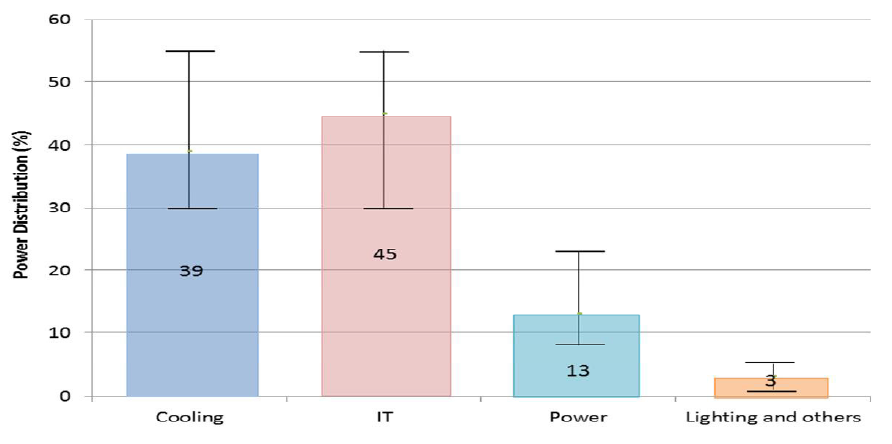
\includegraphics[width=\textwidth]{img/data_center_power_consumption.png}
\caption{Desglose básico de costes en un Datacenter\\\parencite{datacenter_energy_cost_SONG20151255}}
\label{fig:datacenter_energy_cost}
\end{figure}

Esto es una suma monetaria para nada desdeñable, siendo el consumo total de los Datacenter estadounidenses en 2014 de 70TWh (70 mil millones de KWh o \emph{70 billion kWh} en inglés americano),
constituyendo alrededor del 1,8\% del total de consumo de potencia de todos los Estados Unidos en ese mismo año. \autocite[7]{usa_datacenter_energy_usage_report_61109}

Imaginemos por un momento que existe un fabricante que vende modelos más baratos de procesadores, que consumen y disipan menos potencia, y eso se traduce en una bajada de un 10\% en el consumo.
Este pequeño incremento en eficiencia energética se traduce en 7TWh de ahorro energético, por el que muchos datacenters están dispuesto a pagar.

\subsection{Propuesta de valor de ARM}\label{subsection:propuesta_valor_arm}
ARM ofrece un ahorro energético similar al comentado en la sección anterior, pero además también ofrece la posibilidad de licenciar la arquitectura, permitiendo así a grandes compañías
como Amazon, Microsoft y Google crear sus propias CPUs conforme a la \gls{ISA} de ARM, pudiendo cubrir más eficazmente las demandas del dominio de la empresa licenciataria, y ofreciendo aún más
eficiencia energética.

Es en este segundo caso cuando la competencia empieza a ser más evidente entre \gls{x86} y ARM (Figura \ref{fig:graviton_vs_amd_vs_intel_spec_total}), siendo la diferencia en SPECint2017 mononúcleo
positiva para los Amazon Graviton 2 (\ref{subsection:aws_graviton_introduccion}) con respecto
a los AMD EPYC 7571, y rozando a los Intel Xeon Platinum 8259, solo cayendo por poco en SPECfp2017, creando un escenario previsiones muy positivas para la implantación de ARM
en servidores. \parencite{graviton2_vs_amd_vs_intel_cloud_compute}

\begin{figure}[h]
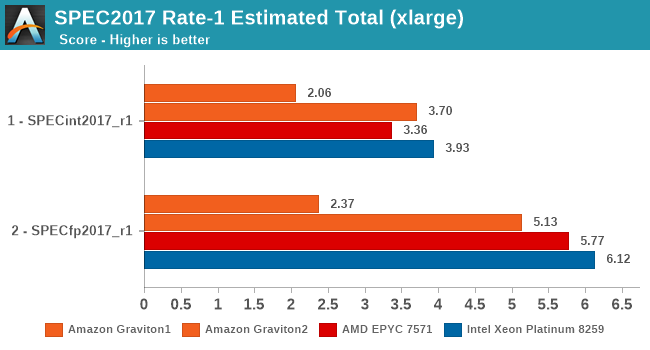
\includegraphics[width=\textwidth]{img/graviton_vs_amd_vs_intel_spec_total.png}
\caption{SPEC2017 Rate-1 Estimated Total}
\label{fig:graviton_vs_amd_vs_intel_spec_total}
\end{figure}


%%%%%%%%%%%%%%%%%%%%%%%%%%%%%%%%%%%%%%%%%%%%%%%%%%%%%%%%%%%%%%%%%%%%%%%%%%%%%%%%%%%%%%%%%%%%%%%%%%%%%%%%%%%%%%%%%%%%%%%%%
%                                                     AWS GRAVITON                                                      %
%%%%%%%%%%%%%%%%%%%%%%%%%%%%%%%%%%%%%%%%%%%%%%%%%%%%%%%%%%%%%%%%%%%%%%%%%%%%%%%%%%%%%%%%%%%%%%%%%%%%%%%%%%%%%%%%%%%%%%%%%
\newpage
\section{AWS Graviton}
\subsection{Introducción}\label{subsection:aws_graviton_introduccion}
Si bien en el el apartado \ref{subsection:propuesta_valor_arm} ya mencionamos las CPU Graviton de Amazon Web Services (AWS Graviton), no se han introducido propiamente aún.

\bigskip

Las CPUs Graviton de Amazon fueron la primera aproximación de la matriz de AWS al diseño propio de CPUs. Basadas en los núcleos \gls{Neoverse}, \gls{IP_intelectual} de ARM, y
diseñados por la compañía israelí subsidiaria de Amazon desde 2015: Annapurna Labs.

Como podemos revisitar en la figura \ref{fig:graviton_vs_amd_vs_intel_spec_total} la primera generación no fue particularmente competente en terminos de rendimiento bruto con respecto a
las opciones de Intel y AMD. Sin embargo con la llegada de la segunda generación de procesadores Graviton, fabricados en nodo de 7nm con respecto a los 16nm de la primera generación
(Figura \ref{fig:aws-graviton2-slide}), el rendimiento ya sí es excelente, permitiendo una rentabilidad nunca antes vista, así como una menor dependencia de Amazon de proveedores
externos. \autocite[]{graviton1_graviton2_zdnet_aws}

\begin{figure}[h]
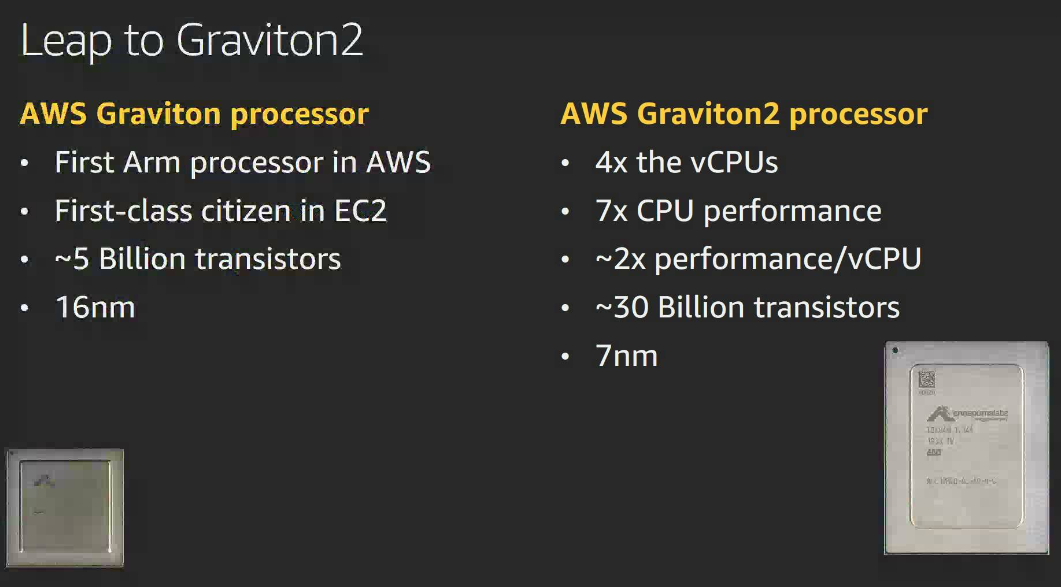
\includegraphics[width=\textwidth]{img/aws-graviton2-slide.png}
\caption{Diapositiva de la Presentación Oficial de AWS Graviton2}
\label{fig:aws-graviton2-slide}
\end{figure}


\subsection{Precios}
Recordemos que los precios de AWS fluctúan bajo demanda, pero más o menos siempre se mantienen dentro de unos márgenes.
A día 13 de Enero del 2021, los precios para las instancias de baja potencia son los siguientes:
\subsubsection{x86: Intel y AMD}
\begin{center}
\begin{tabular}{ | c | c | c | c | }
    \hline
    Tipo de instancia       &   \#CPU   &   RAM [GB]    &   Coste [USD/h]   \\
    \hline
    \texttt{t3a.nano}       &   2       &   0.5         &   0.0047          \\
    \hline
    \texttt{t3.nano}        &   2       &   0.5         &   0.0052          \\
    \hline
    \texttt{t2.nano}        &   1       &   0.5         &   0.0058          \\
    \hline
    \texttt{t3.micro}       &   2       &   1           &   0.0104          \\
    \hline
    \texttt{t2.micro}       &   1       &   1           &   0.0116          \\
    \hline
\end{tabular}
\end{center}

\subsubsection{ARM64: AWS Graviton}
\begin{center}
\begin{tabular}{ | c | c | c | c | }
    \hline
    Tipo de instancia       &   \#CPU   &   RAM [GB]    &   Coste [USD/h]   \\
    \hline
    \texttt{t4g.nano}       &   2       &   0.5         &   0.0042          \\
    \hline
    \texttt{t4g.micro}      &   2       &   1           &   0.0084          \\
    \hline
    \texttt{t4g.small}      &   2       &   2           &   0.0168          \\
    \hline
\end{tabular}
\end{center}

\subsection{Instancias en AWS}\label{subsection:instancias_aws}
La información de las CPUs que se puede encontrar en el Anexo \ref{anexo:info_cpu_aws} y los benchmarks en \ref{subsection:benchmarks_aws} corresponden a
instancias \texttt{t4g.micro} y \texttt{t2.micro} para ARM e Intel respectivamente.

La instancia \texttt{t4g.micro} se ha elegido porque hasta el día 31 de Diciembre del 2020, tenía activa una promoción de prueba gratuita, por lo que si bien no estamos comparando a igualdad
de núcleos físicos, compensaremos esta disparidad en los benchmarks ejecutándolos en modo mononúcleo.

Me parece importante recalcar tambien que aún con el doble de núcleos, la instancia ARM cuesta 0.0084 USD/h, mientras que la instancia x86 son 0.0116 USD/h.

\subsubsection{Diferencias}
Como se puede apreciar, \texttt{t4g.micro}, con menor precio, tiene exactamente las mismas prestaciones que \texttt{t2.micro}, pero dos CPUs, a diferencia de la instancia x86, que solamente tiene uno.
A parte de esto, la información del sistema no tiene por qué decirnos mucho más. No todos los GHz son iguales en la misma familia de procesadores (Por ejemplo un Pentium 4 a 3GHz no rinde
ni de cerca igual que un Ryzen 7 5800X a 3GHz también), y menos entre diferentes familias. Para esto se han ejecutado unos benchmarks muy simples en ambas instancias y medido las diferencias
a continuación.

\subsection{Benchmarks en AWS}\label{subsection:benchmarks_aws}
\subsubsection{Sysbench: Compilación}
Como este programa no se encuentra en los repositorios oficiales, hemos de descargar las dependencias y compilarlo, lo cual nos sirve también como benchmark.

Para esto he creado este pequeño script que realiza todo el trabajo:
\begin{minted}[breaklines]{bash}
    sudo yum -y install git gcc make automake libtool openssl-devel ncurses-compat-libs mysql-devel
    git clone https://github.com/akopytov/sysbench
    cd sysbench
    ./autogen.sh
    ./configure
    make
    sudo make install
\end{minted}

Y los resultados de ejecutar \texttt{time ./script.sh} son los siguientes:
\begin{center}
\begin{tabular}{ | c | c | c | c | }
    \hline
    Arquitectura           &   user        &   sys         &   real        \\
    \hline
    2x ARM64               &   0m49.225s   &   0m3.279s    &   0m55.155s   \\
    \hline
    1x x86                 &   0m57.475s   &   0m4.894s    &   1m10.371s   \\
    \hline
    \hline
    ARM vs x86             &   -16.75\%    &   -49.25\%    &   -27.58\%    \\
    \hline
\end{tabular}
\end{center}

Los cuales dejan en muy buen lugar a ARM, a mi personalente me sorprendió bastante, ya que compilar ARM siempre ha sido notoriamente más lento que x86, pero también partimos con ventaja
de que la instancia ARM tiene dos núcleos vs uno de la x86.

\subsubsection{Sysbench}
El benchmark ha sido realizado en modo mononúcleo, con el siguiente comando:
\begin{minted}{bash}
    sysbench cpu --threads=1 run
\end{minted}

Para no dar una ventaja injusta a la instancia ARM, y los outputs se pueden encontrar en el Anexo \ref{anexo:sysbench_output}, dando lugar
a los siguientes resultados:

\begin{center}
\begin{tabular}{ | c | c | c | c | }
    \hline
    Arquitectura           &   Events/sec  &   Time elapsed &   Total Events    \\
    \hline
    ARM64                  &   2960.7109   &   10.0003s     &   29608           \\
    \hline
    x86                    &   758.0042    &   10.0013s     &   7581            \\
    \hline
    \hline
    ARM vs x86             &   +290.595\%  &   -     &   -    \\
    \hline
\end{tabular}
\end{center}

Los cuales son espectaculares para ARM, teniendo una mejoría de un 290.595\% con respecto a Intel.

Recordemos que estos resultados no se centran en comparar potencia hipotética de una arquitectura, sino comparar dos servicios con un precio similar y observar sus ventajas e inconvenientes.


\subsubsection{7zip}
Para instalar 7zip en Amazon Linux, se han instalado previamente los paquetes:
\begin{minted}[breaklines]{bash}
    sudo amazon-linux-extras install epel
    sudo yum install -y p7zip p7zip-plugins
\end{minted}

De nuevo el benchmark se ha ejecutado en modo mononúcleo, con el siguiente comando:
\begin{minted}[breaklines]{bash}
    7z b -mmt1
\end{minted}
cuyos resultados se pueden encontrar en el Anexo \ref{anexo:7zip_output}, y arrojan los siguientes resultados medios:

\begin{center}
\begin{tabular}{ | c | c | c | }
    \hline
    Arquitectura           &   MIPS Compressing  &  MIPS Decompressing  \\
    \hline
    ARM64                  &   3922              &   3539               \\
    \hline
    x86                    &   3161              &   2754               \\
    \hline
    \hline
    ARM vs x86             &   +24.07\%          &   +25.50\%           \\
    \hline
\end{tabular}
\end{center}

Los cuales de nuevo me han sorprendido. Personalmente pensaba que iba a ganar el procesador x86, pero parece que en estos tiers no se usan CPUs con la suficiente potencia como para
desbancar al procesador Graviton de Amazon, que está portándose increiblemente bien, con una mejoría con respecto al x86 en mononúcleo de un 25\% aproximadamente.


%%%%%%%%%%%%%%%%%%%%%%%%%%%%%%%%%%%%%%%%%%%%%%%%%%%%%%%%%%%%%%%%%%%%%%%%%%%%%%%%%%%%%%%%%%%%%%%%%%%%%%%%%%%%%%%%%%%%%%%%%
%                                                     CONCLUSIONES                                                      %
%%%%%%%%%%%%%%%%%%%%%%%%%%%%%%%%%%%%%%%%%%%%%%%%%%%%%%%%%%%%%%%%%%%%%%%%%%%%%%%%%%%%%%%%%%%%%%%%%%%%%%%%%%%%%%%%%%%%%%%%%
\newpage
\section{Conclusiones}
ARM está entrando con mucha fuerza en el mercado, y estos benchmarks muy reducidos y orientados más bien a los tiers más bajos de AWS parecen confirmarlos: Con ARM podemos obtener más del
doble de rendimiento en AWS por una fracción del precio de x86.

Esto es debido primero al ahorro energético que supone el uso de ARM tanto directa como indirectamente, y segundo debido a que Amazon diseña estos procesadores ``en casa'', por lo que no
necesita sacarles tanto beneficio como por ejemplo Intel con respecto a sus procesadores Xeon.

Sin embargo este cambio no viene sin inconvenientes: Hay programas que no se han portado aún completa o parcialmente para ARM, o que debido al no tan largo recorrido de esta última
arquitectura, no han sido tan optimizados como para la arquitectura x86.
Y es que programar en una arquitectura diferente a la que ejecutará la máquina final es algo que no gusta hacer, pero que con la llegada de ordenadores personales como los nuevos Mac de Apple
(y se espera que de otras marcas), probablemente veremos una explosión de ARM en el mercado de consumo, y por tanto una explosión ciertamente correlacionada en la cantidad de servidores que correrán
sus servicios sobre la microarquitectura de la compañía británica.

\bigskip

La conclusión que yo saco es clara: AWS sobre ARM es más barato que sobre x86, y para algunos ámbitos sin ninguna duda recomendaría su uso, pero quizás para ámbitos donde se necesite más
verificación y seguridad, precisamente por el problema que comentamos de programar en una arquitectura diferente, tambien me siento capaz de afirmar que x86 no va a desaparecer, ni mucho
menos, al menos en el futuro próximo.

Estos benchmarks han de ser tomados con cautela, ya que estamos comparando instancias que no se basan necesariamente en las mismas tecnologías, estando la instancia \texttt{t4g.micro}
basada en el sistema Nitro de AWS, a diferencia de la instancia \texttt{t2.micro}, que es una instancia de rendimiento por ráfagas.

De todos modos estas diferencias no invalidan la conclusión de que, sin ninguna duda, a pesar de que únicamente se ha podido medir de primera mano a pequeñas escala, utilizar instancias de S3
sobre ARM es más económico para Amazon, y por tanto para el cliente final.

\subsection{ARM en Otros Ámbitos}
ARM no solo ha entrado con fuerza en los servicios web de Amazon, si no que el superordenador más potente del mundo según top500 desde el 6 de Junio del 2020 hasta fecha de escritura de este
documento, es el \emph{SUPERCOMPUTER FUGAKU}, fabricado por Fujitsu.
Dicho supercomputador está compuesto por 158.976 CPUs \texttt{A64FX}, con 48 Cores a una frecuencia de 2,2GHz, haciendo uso de innovadoras tecnologías como pueden ser memorias \gls{HBM} integradas en CPU,
una inteligente distribución física de los núcleos, e intercomunicación mediante la tecnología propietaria de Fujitsu: \emph{Tofu Interconnect D}. (\url{https://www.top500.org/system/179807/})

\subsection{Mención Especial: RISC-V}
Con esta parece que inminente transición a paradigmas más basados en RISC, cada vez hay más compañías interesadas en diseñar sus SoCs ``en casa'', y un proyecto que comenzó como universitario
llamado RISC-V está atrayendo bastante atención, sobre todo de las marcas que han de diseñar sus propios chips muy específicos como Western-Digital, Seagate, etc.

De momento a la arquitectura aún le falta mucho ecosistema, pero está entrando con fuerza al conjunto de microarquitecturas que se considerarían viables para uso comercial, existiendo ya
empresas como SiFive. (\url{https://www.sifive.com})

\bigskip

El principal atractivo de RISC-V es que a diferencia de ARM, es una ISA completamente libre de royalties y abierta, lo conocido como ``Open Hardware'', y que probablemente de aquí a unos
años de mucho más de lo que hablar que hoy en día.


\clearpage
\begin{flushleft}
\printbibliography[]{}
\clearpage
\printglossaries
\end{flushleft}


\clearpage
\begin{appendices}
\addappheadtotoc
\appendixpage

%%%%%%%%%%%%%%%%%%%%%%%%%%%%%%%%%%%%%%%%%%%%%%%%%%%%%%%%%%%%%%%%%%%%%%%%%%%%%%%%%%%%%%%%%%%%%%%%%%%%%%%%%%%%%%%%%%%%%%%%%
%                                                        ANEXO 1                                                        %
%%%%%%%%%%%%%%%%%%%%%%%%%%%%%%%%%%%%%%%%%%%%%%%%%%%%%%%%%%%%%%%%%%%%%%%%%%%%%%%%%%%%%%%%%%%%%%%%%%%%%%%%%%%%%%%%%%%%%%%%%
\section{Información de CPU en AWS}\label{anexo:info_cpu_aws}
\subsection{t4g.micro}
\begin{minted}[breaklines]{text}
[ec2-user@ip-172-31-64-28 ~]$ lscpu
Architecture:        aarch64
Byte Order:          Little Endian
CPU(s):              2
On-line CPU(s) list: 0,1
Thread(s) per core:  1
Core(s) per socket:  2
Socket(s):           1
NUMA node(s):        1
Model:               1
BogoMIPS:            243.75
L1d cache:           64K
L1i cache:           64K
L2 cache:            1024K
L3 cache:            32768K
NUMA node0 CPU(s):   0,1
Flags:               fp asimd evtstrm aes pmull sha1 sha2 crc32 atomics fphp asimdhp cpuid asimdrdm lrcpc dcpop asimddp ssbs  

[ec2-user@ip-172-31-64-28 ~]$ cat /proc/cpuinfo | grep processor
processor       : 0
processor       : 1
\end{minted}
\newpage
\subsection{t2.micro}
\begin{minted}[breaklines]{text}
[ec2-user@ip-172-31-60-52 ~]$ lscpu
Architecture:        x86_64
CPU op-mode(s):      32-bit, 64-bit
Byte Order:          Little Endian
CPU(s):              1
On-line CPU(s) list: 0
Thread(s) per core:  1
Core(s) per socket:  1
Socket(s):           1
NUMA node(s):        1
Vendor ID:           GenuineIntel
CPU family:          6
Model:               63
Model name:          Intel(R) Xeon(R) CPU E5-2676 v3 @ 2.40GHz
Stepping:            2
CPU MHz:             2400.104
BogoMIPS:            4800.19
Hypervisor vendor:   Xen
Virtualization type: full
L1d cache:           32K
L1i cache:           32K
L2 cache:            256K
L3 cache:            30720K
NUMA node0 CPU(s):   0
Flags:               fpu vme de pse tsc msr pae mce cx8 apic sep mtrr pge mca cmov pat pse36 clflush mmx fxsr sse sse2 ht syscall nx rdtscp lm constant_tsc rep_good nopl xtopology cpuid pni pclmulqdq ssse3 fma cx16 pcid sse4_1 sse4_2 x2apic movbe popcnt tsc_deadline_timer aes xsave avx f16c rdrand hypervisor lahf_lm abm cpuid_fault invpcid_single pti fsgsbase bmi1 avx2 smep bmi2 erms invpcid xsaveopt

[ec2-user@ip-172-31-60-52 ~]$ cat /proc/cpuinfo | grep processor
processor       : 0
\end{minted}

%%%%%%%%%%%%%%%%%%%%%%%%%%%%%%%%%%%%%%%%%%%%%%%%%%%%%%%%%%%%%%%%%%%%%%%%%%%%%%%%%%%%%%%%%%%%%%%%%%%%%%%%%%%%%%%%%%%%%%%%%
%                                                        ANEXO 2                                                        %
%%%%%%%%%%%%%%%%%%%%%%%%%%%%%%%%%%%%%%%%%%%%%%%%%%%%%%%%%%%%%%%%%%%%%%%%%%%%%%%%%%%%%%%%%%%%%%%%%%%%%%%%%%%%%%%%%%%%%%%%%
\newpage
\section{Sysbench Output}\label{anexo:sysbench_output}
\subsection{Resultados para ARM}
\begin{minted}[breaklines]{text}
[ec2-user@ip-172-31-64-28 sysbench]$ sysbench cpu --threads=1 run
sysbench 1.1.0-bbee5d5 (using bundled LuaJIT 2.1.0-beta3)

Running the test with following options:
Number of threads: 1
Initializing random number generator from current time


Prime numbers limit: 10000

Initializing worker threads...

Threads started!

CPU speed:
    events per second:  2960.71

Throughput:
    events/s (eps):                      2960.7109
    time elapsed:                        10.0003s
    total number of events:              29608

Latency (ms):
         min:                                    0.34
         avg:                                    0.34
         max:                                    0.39
         95th percentile:                        0.34
         sum:                                 9995.37

Threads fairness:
    events (avg/stddev):           29608.0000/0.00
    execution time (avg/stddev):   9.9954/0.00
\end{minted}
\newpage
\subsection{Resultados para Intel}
\begin{minted}[breaklines]{text}
[ec2-user@ip-172-31-60-52 ~]$ sysbench cpu --threads=1 run
sysbench 1.1.0-bbee5d5 (using bundled LuaJIT 2.1.0-beta3)

Running the test with following options:
Number of threads: 1
Initializing random number generator from current time


Prime numbers limit: 10000

Initializing worker threads...

Threads started!

CPU speed:
    events per second:   758.00

Throughput:
    events/s (eps):                      758.0042
    time elapsed:                        10.0013s
    total number of events:              7581

Latency (ms):
         min:                                    1.16
         avg:                                    1.32
         max:                                    5.64
         95th percentile:                        1.37
         sum:                                 9986.84

Threads fairness:
    events (avg/stddev):           7581.0000/0.00
    execution time (avg/stddev):   9.9868/0.00
\end{minted}


%%%%%%%%%%%%%%%%%%%%%%%%%%%%%%%%%%%%%%%%%%%%%%%%%%%%%%%%%%%%%%%%%%%%%%%%%%%%%%%%%%%%%%%%%%%%%%%%%%%%%%%%%%%%%%%%%%%%%%%%%
%                                                        ANEXO 3                                                        %
%%%%%%%%%%%%%%%%%%%%%%%%%%%%%%%%%%%%%%%%%%%%%%%%%%%%%%%%%%%%%%%%%%%%%%%%%%%%%%%%%%%%%%%%%%%%%%%%%%%%%%%%%%%%%%%%%%%%%%%%%
\newpage
\section{7zip Output}\label{anexo:7zip_output}
\subsection{Información de Tiempos}
Como 7zip no arroja información de tiempos de \emph{benchmark}, y debido a la distinta naturaleza de las instancias para ARM y x86, es pertinente especificar que el
tiempo de ejecución de cada uno de estos tests es de \textbf{25 segundos}.

\subsection{Resultados para ARM}
\begin{minted}[breaklines]{text}
[ec2-user@ip-172-31-73-177 ~]$ 7z b -mmt1

7-Zip [64] 16.02 : Copyright (c) 1999-2016 Igor Pavlov : 2016-05-21
p7zip Version 16.02 (locale=en_US.UTF-8,Utf16=on,HugeFiles=on,64 bits,2 CPUs LE)

LE
CPU Freq:  2498  2497  2498  2499  2497  2497  2498  2498  2498

RAM size:     955 MB,  # CPU hardware threads:   2
RAM usage:    435 MB,  # Benchmark threads:      1

                       Compressing  |                  Decompressing
Dict     Speed Usage    R/U Rating  |      Speed Usage    R/U Rating
         KiB/s     %   MIPS   MIPS  |      KiB/s     %   MIPS   MIPS

22:       4213   100   4099   4099  |      41253   100   3522   3522
23:       3808   100   3881   3881  |      40854   100   3536   3536
24:       3567   100   3836   3836  |      40262   100   3535   3535
25:       3393   100   3874   3874  |      40027   100   3563   3563
----------------------------------  | ------------------------------
Avr:             100   3923   3922  |              100   3539   3539
Tot:             100   3731   3731
\end{minted}
\newpage
\subsection{Resultados para Intel}
\begin{minted}[breaklines]{text}
[ec2-user@ip-172-31-60-52 ~]$ 7z b -mmt1

7-Zip [64] 16.02 : Copyright (c) 1999-2016 Igor Pavlov : 2016-05-21
p7zip Version 16.02 (locale=en_US.UTF-8,Utf16=on,HugeFiles=on,64 bits,1 CPU Intel(R) Xeon(R) CPU E5-2676 v3 @ 2.40GHz (306F2),ASM,AES-NI)

Intel(R) Xeon(R) CPU E5-2676 v3 @ 2.40GHz (306F2)
CPU Freq:  2621  2596  2716  2649  2637  2662  2640  2645  2634

RAM size:     983 MB,  # CPU hardware threads:   1
RAM usage:    435 MB,  # Benchmark threads:      1

                       Compressing  |                  Decompressing
Dict     Speed Usage    R/U Rating  |      Speed Usage    R/U Rating
         KiB/s     %   MIPS   MIPS  |      KiB/s     %   MIPS   MIPS

22:       3287   100   3198   3198  |      32298   100   2758   2758
23:       3097   100   3157   3156  |      31826   100   2756   2755
24:       2918   100   3139   3138  |      31603   100   2775   2774
25:       2762   100   3160   3154  |      30675   100   2731   2730
----------------------------------  | ------------------------------
Avr:             100   3164   3161  |              100   2755   2754
Tot:             100   2959   2958
\end{minted}

\end{appendices}

\end{document}